% ---------------------------------------------------------------------------------------------------------
% 学習実験（小規模）
% ---------------------------------------------------------------------------------------------------------
\section{学習実験}
\label{sec:learning}
\subsection{環境とオラクルの整合}
縮約モデルの物理（拘束振り・自由飛行・順応捕捉，摩擦錐，可動域，壁）を CasADi でコード生成・コンパイルした
Gymnasium 環境を用いる（制御周期 20\,ms，積分 RK4 2\,ms，1 コアで数千ステップ/秒）．
関節可動域は軟らかい生理的ストップ（15\,$\tau^{\rm cap}$/rad），指令トルクには最適化器と同じ変化率制限，
捕捉は掛かり線が突起先端の 2.5\,cm 手前から壁までの箱に許容速度で入ったとき指が反射的に閉じる有限剛性フック
（要求力が錐を出ると突起上を滑り，先端を越えると脱落）としてモデル化した．
拘束振りの加速度は最適化器の力学と $10^{-3}$ の相対精度で一致し，オラクル軌道を弱い PD（1/rad，0.1\,s/rad）で追従再生すると，
振り全体で関節角誤差 $\le0.03$\,rad，把持利用率 $U$ は参照値の 3\,\%以内で一致した．
一方，最適解の捕捉は「先端まで 2\,cm・錐制約上」の刃の上にあり，重心の 2--3\,cm のずれで捕捉に失敗する．
これは最適解の非頑健性そのものであり，閉ループ制御と余裕が必要な理由である．

\subsection{双対データとその検証}
表~\ref{tab:costate} に costate の検証を示す．初期条件パラメータの乗数から得た $\partial J^*/\partial\bm x_0$ は
中心差分と \costateFD\,\%で一致し，欠陥制約の乗数から復元した軌道上の costate は，同一問題の初期条件乗数と
最大成分の \costateDense\,\%以内で一致した．したがって 1 本の軌道最適化が $N_S$ 個の状態に双対ラベル
（価値，costate，残り時間，必要容量）を与える．
現時点で \dflNsolve 個の残り最適化問題（うち収束 \dflNok）から \dflNrows 個の状態ラベルを得た．
能力パラメータの影の価格（表~\ref{tab:prices}）は，関節トルク容量の弾性 $\partial\ln J^*/\partial\ln\tau^{\rm cap}$
が中央値 \elastTau（平均 \elastTauMean）と最も大きく，引っ掛かり係数 $\mu_{\rm out}$ がこれに次ぎ，
関節角速度上限と捕捉速度の上限は一度も拘束的でない（価格 0）ことを示す．
容量エピグラフの乗数は保持相に \capHoldShare\,\%，捕捉衝撃に \capCatchShare\,\%，振りに \capSwingShare\,\%が配分され，
必要把持容量を決めているのは振りではなく捕捉後の保持であることが乗数から直接読める．
\begin{table}[t]
\centering\scriptsize
\caption{costate の検証（$T=18$\,s，$m=66$\,kg，振り開始 2.3\,s 後の状態）．}
\label{tab:costate}
\begin{tabular}{lrrrr}
\toprule
成分 & 中心差分 & 乗数（初期条件） & 乗数（欠陥制約，節点外挿） & 相対誤差 \\
\midrule
$\partial J^*/\partial\theta_1$ & 0.1582 & 0.1589 & 0.1625 & 0.4\,\% / 2.3\,\% \\
$\partial J^*/\partial\dot\theta_1$ & --- & $-0.0198$ & $-0.0198$ & $<0.1$\,\% \\
\bottomrule
\end{tabular}
\end{table}
\begin{table}[t]
\centering\scriptsize
\caption{能力パラメータの影の価格 $\partial J^*/\partial\ln p$（残り最適化問題 \dflNok 個の統計）と容量乗数の相別配分．}
\label{tab:prices}
\IfFileExists{tab_prices.tex}{\begin{tabular}{lrrr}
\toprule
パラメータ $p$ & $\partial J^*/\partial\ln p$（中央値） & 平均 & 弾性 $\partial\ln J^*/\partial\ln p$（中央値） \\
\midrule
関節トルク容量 $\tau^{\rm cap}$ & -3.902 & -10.172 & -0.270 \\
引っ掛かり係数 $\mu_{\rm out}$ & -0.147 & -0.326 & -0.010 \\
$\mu_{\rm in}$ & -0.020 & -0.050 & -0.001 \\
関節角速度上限 & 0.000 & 0.000 & 0.000 \\
捕捉相対速度上限 & 0.000 & 0.000 & 0.000 \\
壁から離れる速度上限 & 0.000 & 0.000 & 0.000 \\
\midrule
容量乗数の配分 & 保持 85\% & 捕捉 14\% & 振り 2\% \\
\bottomrule
\end{tabular}
}{（計算中）}
\end{table}

\subsection{双対場の適合と身体間の汎化}
双対場ネットワーク（SiLU，\dflWidth$\times$\dflDepth）を，学習用参照軌道（$m\ne69$\,kg）の 85\,\%で学習し，
残る参照軌道（同じ身体群の未知軌道）と $m=69$\,kg（未知の身体）で評価した（表~\ref{tab:dflfit}）．
価値 $V$ と残り時間 $\tau$ は未知の身体へ $R^2=$\fitVhold，\fitTauhold で汎化し，
costate は Sobolev 項があると $R^2=$\fitPhold，無いと \fitPholdNoSob である．
価値そのものはどちらの学習でも同程度に合うが，その勾配は明示的な双対ラベル無しには学べない．
これは「双対を教師にする」ことの直接の根拠である．
行動模倣（トルク回帰）の未知身体への $R^2$ は \fitUhold であった．
\begin{table}[t]
\centering\scriptsize
\caption{双対場の適合（決定係数）．val：学習身体群の未知参照軌道，holdout：未知の身体（$m=69$\,kg）．}
\label{tab:dflfit}
\IfFileExists{tab_dfl_fit.tex}{\begin{tabular}{llrrrrrr}
\toprule
モデル & 分割 & $n$ & $R^2(V)$ & $R^2(\tau)$ & $\rho_S(\bm p)$ & 符号一致$(\bm p)$ & $R^2(\bm u)$ \\
\midrule
DFL(Sobolev) & train & 24810 & 0.96 & 0.99 & 0.89 & 0.91 & 0.96 \\
DFL(value-only) & train & 24810 & 0.97 & 1.00 & 0.45 & 0.63 & 0.96 \\
DFL(Sobolev) & val & 3944 & 0.73 & 0.95 & 0.73 & 0.82 & 0.69 \\
DFL(value-only) & val & 3944 & 0.71 & 0.96 & 0.41 & 0.64 & 0.69 \\
DFL(Sobolev) & holdout & 5218 & 0.84 & 0.97 & 0.85 & 0.87 & 0.84 \\
DFL(value-only) & holdout & 5218 & 0.90 & 0.99 & 0.46 & 0.65 & 0.84 \\
\bottomrule
\end{tabular}
}{（計算中）}
\end{table}

\subsection{閉ループ：双対場からの制御}
\label{sec:closedloop}
点ごとの Hamiltonian 最小化（Pontryagin 制御器）は，1 制御周期でトルクが価値に与える影響が小さいため
$H$ が $\bm u$ についてほぼ平坦で，costate の 10\,\%程度の誤差で最小点が飽和値へ飛ぶ（条件が悪い）ことが分かった．
オラクル自身の costate を用いても復元トルクの中央値誤差は 0.07，最大 0.6 であり，
最適解のトルクは点ごとの最小化では決まらない（変化率制限と離散化のため）．
そこで，既知の剛体力学を 0.3--0.5\,s 先まで陽に積分し，その終端で双対場を評価する短地平線 MPC
（暗黙 Hermite--Simpson，IPOPT，価値ネットワークを CasADi に埋め込み厳密微分）を双対場の制御器とした．
学習した価値場をそのまま終端コストにすると，MPC はデータの外で価値が低く外挿された状態を「発見」して
そこへ向かう（0.3\,s 先で $V_\vartheta$ が 2--3 低い状態；学習器と最適化器の敵対）．
4 個の場のアンサンブル（平均$+2\sigma$）だけでは外挿の一致のため防げず，
学習データの混合ガウス密度による分布外ペナルティを終端に加えることで初めて価値の搾取が止まった．
執行側では，オラクル解が引っ掛かり錐と可動域の境界上にあるため，計画の錐を 25\,\%＋絶対値 0.03\,$F_{\rm cap}$ だけ
内側に締め（制約タイトニング），最初の指令を現在の指令に変化率制限で結ぶ必要があった．
比較のため，同じ執行系で (i)~行動模倣（BC），(ii)~双対場 MPC，(iii)~オラクルを 0.4--0.5\,s ごとに解き直す
オラクル・イン・ザ・ループ MPC（計算量の上限；1 エピソード 10--40 分）を評価した（表~\ref{tab:dflcl}）．
\begin{table}[t]
\centering\scriptsize
\caption{閉ループ評価（$T=18$\,s，$m\in\{60,\dots,75\}$\,kg の参照解，静止開始＋摂動開始）．
生存時間は失敗までの時間，離手率は離手に至ったエピソードの割合．}
\label{tab:dflcl}
\IfFileExists{tab_dfl_closedloop.tex}{\begin{tabular}{lrrrrrrrl}
\toprule
制御器 & $n$ & 離手 & 捕捉 & 保持（成功） & 最接近中央値 [cm] & 生存時間中央値 [s] & $\Upk$ 中央値 & 主な失敗 \\
\midrule
行動模倣（BC） & 10 & 0\% & 0\% & 0\% & --- & 2.7 & 0.84（$U^*$=1.14） & A で滑り \\
双対場 MPC（$V$ 終端，0.3\,s） & 10 & 0\% & 0\% & 0\% & --- & 2.3 & 1.15（$U^*$=1.14） & 壁に接触 \\
双対場 MPC（$V$ 終端，0.8\,s） & 10 & 10\% & 0\% & 0\% & 232.9 & 2.7 & 1.23（$U^*$=1.14） & A で滑り \\
双対場 MPC（$V$＋$\tau$ 進行，0.3\,s） & 10 & 0\% & 0\% & 0\% & --- & 2.8 & 1.35（$U^*$=1.14） & 壁に接触 \\
双対場 MPC（$V$＋$\tau$ 進行，初期制約緩和） & 10 & 0\% & 0\% & 0\% & --- & 9.0 & 1.55（$U^*$=1.14） & 壁に接触 \\
双対場 MPC（$V$＋$\tau$ 進行，計画の PD 追従） & 9 & 0\% & 0\% & 0\% & --- & 5.4 & 1.19（$U^*$=1.14） & A で滑り \\
オラクル MPC & 10 & 100\% & 40\% & 10\% & 3.8 & 5.7 & 1.36（$U^*$=1.14） & B 前面に衝突 \\
\bottomrule
\end{tabular}
}{（計算中）}
\end{table}
\closedloopSummary

\subsection{強化学習との比較}
同じ環境・同じ着地反射で PPO（8 並列環境，300 万ステップ）を，疎報酬，振りエネルギー整形，
最接近距離整形，双対価格整形の組合せについて学習させた（図~\ref{fig:rl}）．
初期の報酬設計では「早く死ぬ」「即離手」「期限まで静止」の三つの局所解が順に現れ，
早期失敗ペナルティ・指令変化率制限・離手閾値の導入後は全条件が「期限まで静止」（報酬 $-109$〜$-121$）に収束し，
300 万ステップで成功は一度も観測されなかった（\rlSuccessAll 回/\rlEpisodesAll エピソード）．
参照状態初期化（DeepMimic 型）を加えると離手は生じるが捕捉には至らない．
本課題では疎な成功信号に基づく方策探索は，密な双対情報（価値・costate・価格）を持つオラクル駆動の学習より
はるかに非効率であることが，同一環境で確認された．
\IfFileExists{../results/figs/rl_curves.pdf}{%
\begin{figure*}[t]
\centering
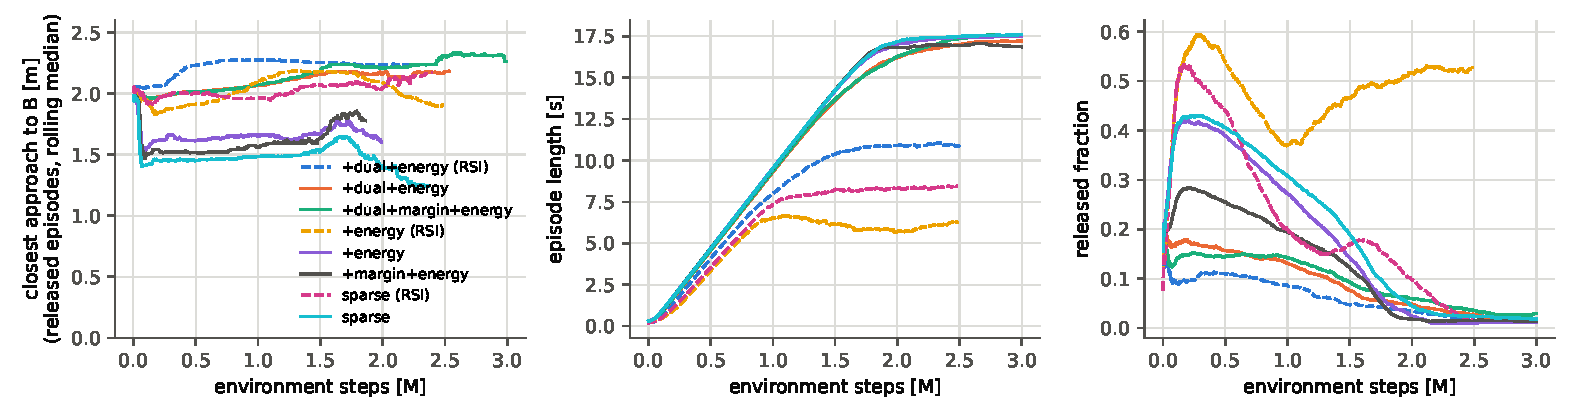
\includegraphics[width=\linewidth]{../results/figs/rl_curves.pdf}
\caption{PPO の学習曲線（移動平均）：成功率，エピソード長，離手率．}
\label{fig:rl}
\end{figure*}}{}
